\documentclass{comjnl}

\usepackage{amsmath}

\usepackage{pagecolor}
%\copyrightyear{2009} \vol{00} \issue{0} \DOI{000}

% for full width figures\
\usepackage{lipsum}% http://ctan.org/pkg/lipsum
\usepackage{graphicx}% http://ctan.org/pkg/graphicx

% random
\usepackage[utf8]{inputenc} % allow utf-8 input
\usepackage[T1]{fontenc}    % use 8-bit T1 fonts
\usepackage{hyperref}       % hyperlinks
\usepackage{url}            % simple URL typesetting
\usepackage{nicefrac}       % compact symbols for 1/2, etc.

% double column box
\usepackage{cuted,tcolorbox,lipsum}

% code embeds
\usepackage{listings}
\usepackage{color}

\definecolor{dkgreen}{rgb}{0,0.6,0}
\definecolor{gray}{rgb}{0.5,0.5,0.5}
\definecolor{mauve}{rgb}{0.58,0,0.82}

\lstset{frame=tb,
  language=Go,
  aboveskip=3mm,
  belowskip=3mm,
  showstringspaces=false,
  columns=flexible,
  basicstyle={\small\ttfamily},
  numbers=none,
  numberstyle=\tiny\color{gray},
  keywordstyle=\color{blue},
  commentstyle=\color{dkgreen},
  stringstyle=\color{mauve},
  breaklines=true,
  breakatwhitespace=true,
  tabsize=3
}

% color the json
\lstdefinelanguage{json}{
  basicstyle={\small\ttfamily},
  numbers=none,
    numberstyle=\scriptsize,
    stepnumber=1,
    numbersep=8pt,
    showstringspaces=false,
    breaklines=true,
    frame=lines,
    backgroundcolor=\color{white},
    literate=
     *{0}{{{\color{black}0}}}{1}
      {1}{{{\color{black}1}}}{1}
      {2}{{{\color{black}2}}}{1}
      {3}{{{\color{black}3}}}{1}
      {4}{{{\color{black}4}}}{1}
      {5}{{{\color{black}5}}}{1}
      {6}{{{\color{black}6}}}{1}
      {7}{{{\color{black}7}}}{1}
      {8}{{{\color{black}8}}}{1}
      {9}{{{\color{black}9}}}{1}
      {:}{{{\color{gray}{:}}}}{1}
      {\{}{{{\color{gray}{\{}}}}{1}
      {\}}{{{\color{gray}{\}}}}}{1}
      {[}{{{\color{gray}{[}}}}{1}
      {"}{{{\color{gray}{"}}}}{1}
      {,}{{{\color{gray}{,}}}}{1}
      {]}{{{\color{gray}{]}}}}{1},
}


\usepackage{trivfloat}
\trivfloat{example}

\begin{document}
\pagecolor{white}


\title[An event-sourced and distributed database with IPLD and materialized views]{An event-sourced and distributed database with IPLD and materialized views}
\author{Pick}
\author{Farmer}
\author{Sutula}
\author{Hill}
\affiliation{www.textile.io} \email{contact@textile.io}

\shortauthors{www.textile.io}

\revised{18 September 2019}


%\category{C.2}{Computer Communication Networks}{Computer Networks}
%\category{C.4}{Performance of Systems}{Analytical Models}
%\category{G.3}{Stochastic Processes}{Queueing Systems}
%\terms{Internet Technologies, E-Commerce}
\keywords{Databases; Event Sourcing; IPFS; IPLD}


\begin{abstract}
As the Internet expands, the division between a person's digital and physical existence continues to blur. An emerging issue of concern is that the digital part of a person's life is mainly being captured by apps and stored away from the person’s control by the companies building those apps. An alternative, called user-siloed data is an exciting area of research that if implemented successfully, could reverse the flow of value derived from personal data, from apps to users. In this paper, we investigate the data formats, and storage and transfer protocols necessary to build a system for user ownership of large-scale digital datasets. The aim of the proposed system is to help power a new generation of web technologies. Our solution combines a novel use of event sourcing with Interplanetary Linked Data (IPLD) to provide a distributed, scalable, and flexible database solution for decentralized applications.
\end{abstract}

\maketitle


\section{Introduction}

Compared to their predecessors, modern cloud-based apps and services provide an extremely high level of convenience. Users can entirely forget about the risk of data loss and enjoy seamless access to their apps across multiple devices. This convenience is now expected, but has come at the cost of additional consequences for users. One such consequence is that many of the same development patterns that bring convenience (e.g., single sign-on, minimal encryption, centralized servers, and databases) also enable or even require data hoarding by the apps. While collecting large amounts of user’s data can create value for the companies building apps (e.g., app telemetry, predictive tools, or even new revenue streams), that value flows mostly in one direction; Apps collect, process and benefit from a user's private data, but users rarely have access to the original data or the new insights that come from it. Additionally,  the data may not be readily accessible to other apps and services. This is app-siloed data.

While companies collecting user data may not be itself a significant problem, it has been shown that over time company incentives often shift from providing value to users to extracting value from users [ref Dixon]. When this incentive shift happens for companies that have also been hoarding user data, that data may be a new source of value or even revenue for the company. It may be possible to stop this trend through extreme privacy measures, government intervention/legislation, or by boycotting companies that collect any form of data. Ideally, there is an alternative approach that allows individuals to capture the value of their data and still allow developers to build new interfaces and experience on top of this data. This approach is called user-siloed data and it fundamentally separates apps from their user’s data.

One of the most exciting aspects of user-siloed data is the the ability to build data-driven apps and services while users remain in control of their own data. Other projects have identified app silo-ed data as a problem [ref], and some have identified user-siloed data as a solution [ref Solid]. However, none so far have provided a sufficiently interoperable protocol for scalable storage and transmission of user-siloed application data. This is the key to building great applications on user-siloed data.

In this paper, we study existing technologies that could be used to build a network for user-siloed data. We outline six challenge areas: flexible data format, efficient synchronization, conflict resolution, access-control, scalable storage, and network communication. Based on our findings, we propose a novel architecture for event sourcing with Interplanetary Linked Data (IPLD), designed to store, share, and host user-sioled datasets at scale. Our proposed design leverages new and existing protocols to solve major challenges involved with building a secure and distributed network for user data while at the same time providing the flexibility and scalability required by today's applications. 


\section{Background}
\label{sec:Background}

We now describe some of the technologies and concepts motivating the design of our novel distributed database system. We highlight some of the advantages and lessons that can be learned from event-sourcing and discuss drawbacks to using these approaches in distributed systems. We provide an overview of some important technologies related to IPFS that make it possible to rethink event sourcing in a decentralized network. Finally, we cover challenges of security and access control on an open and decentralized network and discuss how they are used in popular databases external to IPFS. 

\subsection{Data Synchronization}

\subsubsection{CQRS, Event Sourcing, and Logs}

When developing large-scale software systems, it is common to store data in a relational database management system (RDBMS). To model realistic systems, this type of framework often requires complex techniques for mapping data between domain models and database tables, where the same data model is used to both query and update a database. An powerful alternative is to use a set of append only logs to model the state of an object simply by applying its change sequence in the correct order. This concept can be expressed succinctly by the state machine approach [ref]: if two identical, deterministic processes begin in the same state and get the same inputs in the same order, they will produce the same output and end in the same state. This is a powerful concept baked into a simple structure, and is at the heart of many distributed database systems [ref].

\begin{definition} (Logs or Append-only log). A log is a registry of database transactions that is read sequentially (normally ordered by time) from beginning to end. In distributed systems, logs are often treated as append-only, where changes or updates can only be added to the set and never removed.  \end{definition} \label{def:Logs}

In modern applications it is critical to have reliable mechanisms for publishing updates and events (i.e., to support event-driven architectures), scalability (optimized write and read operations), forward-compatible application updates (e.g., code changes, retroactive events, and others), auditing systems, etc. To support such requirements, developers have begun to utilize event sourcing and command query responsibility segregation (CQRS) patterns [ref], relying on append only logs to support immutable state histories. Indeed, a number of commercial and open source software projects have emerged in recent years that facilitate event sourcing and CQRS-based applications, including Event Store [ref], Apache Kafaka [ref] and Samza [ref], among others [see ref]. 

\begin{definition} (Command query responsibility segregation). Command query responsibility segregation or CQRS is a design pattern whereby reads and writes are separated into different models, using commands to write data, and queries to read data [ref]. \end{definition}

\begin{definition} (Event sourcing). Event sourcing (ES) is a design pattern for persisting the state of an application as an append-only log of state-changing events. \end{definition}

ES is particularly useful in contexts where system components are distributed or decentralized, such as in decentralized applications (DApps). This is because the design of systems that use event sourcing often necessitate infrastructure for brokering messages between loosely coupled software components and services. This feature will become increasingly important as we outline background concepts related to data synchronization in the following sections. 

A key principal of ES and append only logs is that all changes to application state are stored as a sequence of events. Because any given state is simply the result of a series of atomic updates, the log can be used to reconstruct past states or process retroactive updates [ref]. The same principal means a log can be viewed as a mechanism to support an infinite number of valid state interpretations (see section  \ref{sec:ViewsProjections}). In other words, with minimal conformity, a single log can model multiple application states [ref].

\subsubsection{Views \& Projections} \label{sec:ViewsProjections}

\begin{definition}  (View). A (typically highly de-normalized) read-only model of the data. Views are tailored to the interfaces and display requirements of the application, which helps to maximize both display and query performance. Views that are backed by a database or filesystem-optimized access are referred to as materialized views. \end{definition}

\begin{definition} (Projection). An event handler and corresponding reducer/fold function used to build and maintain a view from a set of (filtered) events. While projections may lead to the generation of new events, their reducer should be a pure function (see [ref] and [ref] for examples from existing systems). \end{definition}

In CQRS and ES, the separation of write operations from read operations is a powerful concept. It allows developers to define views into the underlying data that are best suited for the use case or user interface they are building. Multiple views can be built from the same underlying event log, and they can be quite different from one another.

Views themselves are enabled by projections. Projections can be thought of as transformations or reducers that are applied to each event in a stream of events. They update the data backing the views, be this in memory, or persisted to a database. In a distributed setting, it may be necessary for projections to define and operate as eventually consistent data structures, to ensure all peers operating on the same stream of events have a consistent representation of the data.

\subsubsection{Eventual Consistency} \label{sec:EventualConsistency}

The CAP theorem [ref, ref] states that a distributed database can guarantee only two of the following three promises at the same time: consistency (i.e., that every read receives the most recent write or an error), availability (i.e., that every request receives a (possibly out-of-date) non-error response, and partition tolerance (i.e., that the system continues to operate despite an arbitrary number of messages being dropped (or delayed) by the network). As such, many distributed systems are now designed to provide availability and partition tolerance by trading consistency for eventual consistency. Eventual consistency allows state replicas to diverge temporarily, but eventually arrive back to the same state again. While an active area of research, designing systems with provable eventual consistency guarantees remains challenging [ref needed].


\begin{definition} (CRDT). A conflict-free replicated data type (CRDT) assures eventual consistency through optimistic replication (i.e. all new updates are allowed) and eventual merging. CRDTs rely on data structures that are mathematically guaranteed to resolve concurrent updates the same way regardless of the order those events were received. \end{definition} \label{def:CRDT}

How a system provides eventual consistency is often decided based on the intended use of the system. Two well-documented categories of solutions include logs (see Definition  \ref{def:Logs}), sequences of deterministic changes, and CRDTs (see Definition section  \ref{def:CRDT}). Logs work best when there is only a single-writer or complete event causality is known. In many distributed systems with multiple log writers, a minimum requirement for synchronization through logs is that the essential order of events is respected and can be determined [3, 8]. For these cases, logical clocks are a useful tool for eventual consistency and total ordering [ref]. However, some scenarios (e.g., temporarily missing events, or ambiguous order) can force a replica into a state that cannot be later resolved without costly recalculation. In specific cases, CRDTs can provide an alternative to log-based consensus (see below). 

\subsubsection{Logical Clocks}

In a distributed system, where multiple machines, each with an independent clock, are creating events, local timestamps can’t be used to construct global event causality. Machine clocks are never perfectly synchronized [1], meaning that one machine's concept of "now" is not necessarily the same as another machine's. Machine speed, network speed, and other factors compound the issue. For this reason, simple wall-clock time does not provide a sufficient notion of order in a distributed system. Alternatives to wall-clock time exist to help distributed systems achieve eventual consistency. Examples include various logical clocks (Lamport [ref below], Schwartz [ref below], and Bloom [ref below], Hybrid variants [ref below], etc), which use counter-based time-stamping to provide partial ordering. 

Cryptographically linked events can also represent a clock. One such example is called the Merkle-Clock [ref below]. The Merkle-Clock relies on properties of a Merkle-DAG to provide strict partial ordering between events, which has limitations [ref section 4.3 of the merkle paper]:

\begin{quote}
Merkle-Clocks represent a strict partial order of events. Not all events in the system can be compared and ordered. For example, when having multiple heads, the Merkle-Clock cannot say which of the events happened before.
\end{quote}

See Section \ref{sec:merkleclocks}.

\subsubsection{Conflict-Free Replicated Data Types}

In distributed models that use clock-based ordering as described above, a replica can arrive in a state that will require conflict resolution through consensus or rollback. Those operations can be expensive, having adverse effects on the scalability of distributed systems, especially ones attempting to synchronize an application state. 

CRDTs (see Definition \ref{def:CRDT}) are one way to achieve strong eventual consistency, where once all replicas have received the same events, they will arrive at the same final state, regardless of ordering. A review of the types of possible CRDTs is beyond the scope of this paper, however, it is important to note their role in eventually consistent systems and how they relate to clock-based event ordering. See for example [Merkle Clock ref] and [ref] for informative reviews of these types of data structures.

Whether a system (e.g., an app) uses a CRDT or a clock-based sequence of events is entirely dependent on the use-case and final data model. While CRDTs may seem superior (and are currently a popular choice among decentralized systems), it is not possible to model every system as a CRDT. Additionally, the simplicity of clock-based sequencing often makes it easier to leverage in distributed systems where data conflicts will only rarely arise. Lastly, logs and CRDTs are not mutually exclusive and can be used together or as different stages of a larger system.

\subsection{Content-based addressing}

Internet application architecture today is often designed as a system of clients (users) communicating to endpoints (hosts). Communication between clients and endpoints (servers) happens via the TCP/IP protocol stack and therefore largely relies on a mechanism referred to as location-based addressing. Location-based addressing, where the client makes a request that is routed to a specific endpoint based on prior knowledge (e.g., the domain name or IP address), works relatively well for many use-cases. However, there are many reasons why addressing content by location is problematic, such as duplication of storage, inefficient use of bandwidth, link rot, centralized control, and authentication issues. An alternative to location addressing, called content addressing may provide a solution to those problems. Content addressing is where the content itself is used to create an address and retrieve that content from a network [2].

\subsubsection{IPFS \& Content-based addressing}

There are a number of systems that utilize content addressing to access content and information [list some as refs], and there is an active body of literature covering its design and implementation [ref]. The Interplanetary File System (IPFS) — which is a set of protocols to create a content-addressed, peer-to-peer filesystem [1] — is one such system. In IPFS, the address for any content is determined based on a cryptographic hash of the content itself. In practice, the IPFS Content IDentifier (CID) is a multihash, which is a self-describing “protocol for differentiating outputs from various well-established cryptographic hash functions, addressing size + encoding considerations” [ref]. That addressing system confers several benefits to the network, including tamper resistance (we can be confident that a given piece of content has not been modified en route if its hash matches what we were expected/requested) and de-duplication (because the same content from different peers will produce the same hash address). Additionally, IPFS content addresses are immutable and universally unique.

\begin{figure}
  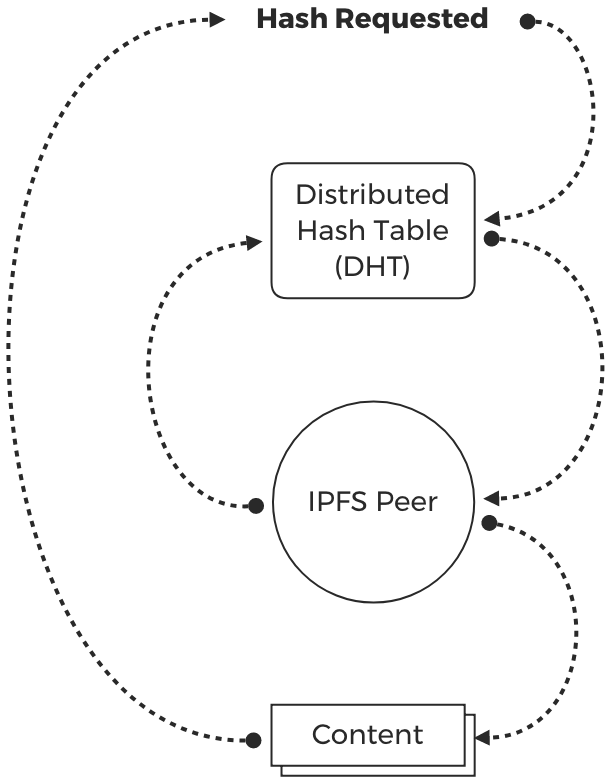
\includegraphics[width=\linewidth]{figures/Hash_Request.png}
  \caption{The crypographic hash of content is used to make a request to the network of IPFS peers. Using the built-in routing machanisms and the distributed hash table, a peer(s) hosting the requested content is identified and content is returned. }
  \label{fig:contentaddressing}
\end{figure}

While content addressing doesn’t tell you how to get a file, IPFS (via libp2p [ref]) provides a system for moving files across the network.  On the IPFS network, a client who wants specific content requests the CID from the network of IPFS hosts. The client's request is routed to the first host capable of fulfilling the request — i.e., the first host that is actively storing the content behind the given CID. The IPFS network can be seen as a distributed file system, with all of the benefits [ref] that come with this type of file system design.


\subsubsection{IPLD}

As discussed above, IPFS uses the cryptographic hash of a given piece of content to define its content address (see [ref] for details on this process). However, in order to provide standards for accessing content-addressable data (on the web or elsewhere), it is necessary to define a common format or specification. In IPFS (and other projects [ref]), this common data format is called Interplanetary Linked Data (IPLD) [ref]. As the name suggests, IPLD is based on principals of linked data [ref, ref] with the added capabilities of a content-addressing storage network. 

IPLD is used to publish linked data (subject-predicate-object triples in the linked data world [ref]) spread across different hosts, and where everything (entities, predicates, data sources) uses content addresses as unique identifiers [ref]. To form its structure, IPLD implements a Merkle DAG, or directed acyclic graph. This allows all hash-linked data structures to be treated using a unified data model, analogous to linked data in the Semantic Web sense [ref]. In practice, IPLD is represented as objects, each with `Data` and `Links` fields, where `Data` can be a small blob of unstructured, arbitrary binary data, and `Links` is an array of links to other IPLD objects. 

\subsubsection{Merkle-Clocks} \label{sec:merkleclocks}

A Merkle-Clock is a Merkle-DAG that represents a sequence of events. In other words, a Merkle-Clock is an append-only log [ref and ipfs-log]. When implemented on IPFS (or an equivalent network where content can be cryptographically addressed and fetched), Merkle-Clocks provide a number of benefits for data synchronization between replicas [ref merkle paper section 4.3]:

\begin{enumerate}
\item \label{Perf1}Broadcasting the Merkle-Clock requires broadcasting only the current root CID. The whole Clock is unambiguously identified by the CID of its root and its full DAG can be walked down from it as needed.
\item \label{Perf2}The immutable nature of a Merkle-DAG allows every replica to perform quick comparisons and fetch only those nodes that it does not already have.
\item \label{Perf3} Merkle-DAG nodes are self-verified and immune to corruption and tampering. They can be fetched from any source willing to provide them, trusted or not.
\item \label{Perf4} Identical nodes are de-duplicated by design: there can only be one unique representation for every event.
\end{enumerate}

On the downside, and as seen above (section 2.2.4.), a Merkle-Clock cannot order divergent heads (or roots):

\begin{figure}
  
\includegraphics[width=\linewidth]{boat.jpg}
  \caption{Divergent heads in a multi-writer Merkle-DAG }
  \label{fig:merkledag}
\end{figure}

In the figure above, two replicas (top row, bottom row) are attempting to write (left to right) events to the same Merkle-Clock. After the first replica writes event A, the second writes event A’ and properly links to A. At that point, the two replicas stop receiving events from one another. To a third replica that does continue to receive events, there would now be two independent heads, 1 and 1’. For the third replica, resolving these two logs of events may be costly (many updates happened since the last common node) or impossible (parts of the chain may not be available on the network). See Section  \ref{sec:EventualConsistency}.

In order to reduce the likelihood of divergent heads, all replicas should be perfectly connected and be able to fetch all events and linkages in the Merkle-Clock. On real networks with many often offline replicas (mobile and IoT devices, laptops, etc.), these conditions are rarely met.

Based on these observations, using a single Merkle-Clock to synchronize replicas can be problematic.

\subsection{Networking}

So far we have primarily discussed the mechanics of creating or linking content in a series of updates. Now we will overview some common networking tools for connecting distributed peers who aim to maintain replicas of a shared database. This could be any decentralized network of interacting entities (e.g., cloud servers, IoT devices, botnets, sensor networks, mobile apps, etc) collectively updating a shared state. IPFS contains a collection of protocols and systems to help address the networking needs required by different use-cases. That is to say no matter what type of device we are talking about — be it a phone, desktop computer, browser, or Internet-enabled appliance — it should be able to communicate with other devices. However, each of the networking approaches described below comes with strengths and weaknesses when used to synchronize data.

\subsubsection{Libp2p}

The libp2p project provides a robust protocol communication stack. IPFS and a growing list of other projects [ref] are building on top of libp2p. Libp2p solves a number of challenges that are distinct to peer-to-peer (p2p) networks. A comprehensive coverage of networking issues in P2P systems is out of the scope for this paper, however, some core challenges that libp2p helps to address include NAT traversal, peer discovery and handshake protocols, and even encryption and transport security — libp2p supports both unencrypted (e.g. TCP, UDP) and encrypted protocols (e.g. TLS, Noise) — among others. Libp2p uses the concept of a multiaddress to address peers on a network, which essentially models network addresses as arbitrary encapsulations of protocols [ref, ref]. In addition to “transport layer” modules, libp2p provides several tools for sharing and/or disseminating data over a p2p network.

\subsubsection{Pubsub}

One of the most commonly used p2p distribution layers built on libp2p, is its Pubsub (or publish-subscribe) system. Pubsub is a standard messaging pattern where the publishers don’t know who, if anyone, will subscribe to a given topic. Publishers send messages on a given topic or category, and Subscribers receive only messages on a give topic they are subscribed to. Libp2p’s pubsub module can be configured to utilize a floodsub protocol — which floods the network with messages, and peers are required to ignore messages they are not interested in — or gossipsub — which is a proximity-aware epidemic pubsub, where peers communicate with proximal peers, and messages can be routed more efficiently. In those implementations, there is a benefit to using pubsub in that no direct connection between publishers and subscribers is required.

Another benefit to using pubsub is the ability to publish topical sequences of updates to multiple recipients. Like libp2p, encryption is a separate concern and often added in steps prior to data transmission. However, like libp2p, pubsub doesn’t offer any simple solutions for transferring encryption keys (beyond public keys), synchronizing datasets across peers (i.e. they aren’t databases), or enforcing any measures for access control (e.g. anyone subscribed to a topic can also author updates on that topic). To solve some of those challenges, some systems introduce message echoing and other partial solutions. However, it makes more sense to use pubsub and libp2p as building blocks in systems that can effectively solve these issues, by choosing multi-modal communication strategies or leveraging tools such as deferred routing (e.g. inboxing) for greater tolerance of missed messages.

\subsubsection{IPNS}

Pubsub and libp2p have so far dealt with the push transfer of data, but IPFS also offers a useful technology for hosting pull/request based data endpoints called, IPNS. IPNS aims to address the challenge of mutable data within IPFS. IPNS relies on a global namespace (shared by participating IPFS peers) based on Public Key Infrastructure. By using IPNS, a content creator generates a new address in the global namespace and points that address to an endpoint (e.g. a CID). Using their private key, a content creator can update what static route the IPNS address refers to. IPNS isn’t only useful for creating static addresses that can point to content addresses, IPNS is compatible with a naming system external from IPFS, such as DNS, onion, or bit addresses. However, many use-cases that require highly mutable data, require rapid availability of updates, or want flexible multi-party access control may not yet be suitable for IPNS. Taken together, libp2p, pubsub, IPNS, and IPFS more generally provide a useful toolkit for building robust abstractions to deliver fast, scalable, data synchronization in the decentralized network. 


\subsection{Data Access \& Control}

\subsubsection{Identity}

IPFS is an implementation of public key infrastructure, where every node on the IPFS network has a key-pair. In addition to using the key-pair for secure communication between nodes, IPFS also uses the key-pair as the basis for identity. Specifically, when a new IPFS node is created, a new key-pair is generated, and then the public key is transformed into the nodes Peer ID. 

\subsubsection{Agent-centric security}

Agent-centric security refers to the practice of maintaining data integrity without leveraging a central or blockchain-based consensus. The general approach is just to let the reader enforce permissions and perform validations, not the writer or some central authority. Agent-centric security is possible if the reader can reference local-only, tamper-free code or if the state can be used to determine whether a given operation (e.g. delete data) is permitted. Many decentralized networks like Secure Scuttlebutt [1] and Holochain [2] make use of agent-centric security. Each of these systems leverage cryptographic signatures to validate peer identities and messages.


\subsubsection{Access control}

All filesystems and databases have some notion of "access control." Many make use of an access-control list (ACL), which is a list of permissions attached to an object or group of objects [ref]. An ACL determines which users or processes can access an object and whether a particular user or process with access can modify or delete the object. 

\begin{figure}
  
\includegraphics[width=\linewidth]{boat.jpg}
  \caption{Example Access Control List.}
  \label{fig:boat1}
\end{figure}

Using ACLs in systems where identity is derived from various configurations of public-key infrastructure has been around for some time [1, 2]. Still, many existing database and communication protocols built on IPFS to date lack support for an ACL or only have primitive ACL support. Where ACLs are missing, many systems use cryptographic primitives like signature schemes or enable encryption without any role-based configuration. Even more, many systems deploy an all-or-none security model, where those with access to a database have complete access, including write capabilities. ACLs should be mutable over time and permission to modify an ACL should also be recorded in an ACL.

Event-driven systems (e.g., event sourcing) often make use of ACLs with some distinct properties. The ACL of an event-driven system is usually a list of access rules built from a series of events. For example, the two events, "grant Bob write access" and "revoke read access from Alice" would together result in a final ACL state where, Bob has read and write access, but Alice does not (see Section  \ref{sec:ViewsProjections}).


\section{The Threads protocol}

We propose Threads, a protocol and decentralized database that runs on IPFS meant to help decouple apps from user-data. The Threads protocol is designed based on an underlying, CQRS-inspired event-sourcing system for synchronizing data across collaborating peers on a network. Threads offer data ownership and a multi-role data access architecture where owners can set independent permissions for writing, reading, and following data updates. Threads differ from previous solutions by extending on the multiaddress addressing scheme to allow PULL based replica synchronization in addition to more common PUSH based synchronization seen in decentralized protocols. The flexible event-based structure enables client applications to model advanced states through aggregates, views, and custom CRDTs.

Threads are topic-based collections of single-writer logs. Taken together, these logs represent the current “state” of an object or dataset. The basic units of Threads, namely Logs and Events, provide a framework for users to create, store, and transmit data in a P2P distributed network. By structuring the underlying architecture in specific ways, this framework can be deployed to solve many of the problems discussed above.

\subsection{ Event Logs}

\subsubsection{Single-writer Event Logs}

In multi-writer systems, determining causal order in all replicas is particularity challenging. As previously discussed (section 2.2.4), a solution based on a Merkle-Clock is only partially ordered. That is, this approach cannot achieve a total order of events without implementing a data-layer conflict resolution strategy [ref]:


\begin{quote}
	A total order can be useful ... and could be obtained, for example, by considering concurrent events to be equal. Similarly, a strict total order could be built by sorting concurrent events by the CID or their nodes or by any other arbitrary user-defined strategy based on additional information attached to the clock nodes (data-layer conflict resolution).
\end{quote}

In many cases, the total order of an event sequence is meaningful, and this type of deterministic merge strategy in not sufficient. A git merge highlights one such case, in which additional information is sometimes needed in order to resolve a line conflict. Ledger based transactions present a similar challenge where the absolute order of transactions between multiple peers really does matter.

Our solution to deal with divergent Merkle-Clocks is to institute a single-writer rule: A log can only be updated by a single replica or identity. An Event Log is a single-writer Merkle-Clock that can be totally ordered. Separate Event Logs can be composed into advanced structures, including CRDTs [Ref Enes].

Practically speaking, for any given Log, Events are authored by a single IPFS Peer, or Writer.

\begin{definition}
(Writer). The single IPFS Peer capable of writing to an Event Log.
\end{definition}

This single-writer setup is a core feature of Logs, and provides properties unique to the Threads protocol. For clarity, we can similarly define a Reader as any other Peer capable of reading a Log.

\begin{definition}
(Reader). Any Peer capable of reading a Log. Practically speaking, this means any Peer with the Log’s Read key (see Section  \ref{sec:KeysEncryption}).
\end{definition}


As seen above in section 2.3.4., a Merkle-Clock is simply a Merkle-DAG of Events:

\begin{definition}
 (Event). An single node in a Merkle-Clock, stored on IPFS.
\end{definition}

\begin{figure}
  
\includegraphics[width=\linewidth]{boat.jpg}
  \caption{A single-writer Merkle-Clock (Event Log).}
  \label{fig:boat1}
\end{figure}

Together with a cryptographic signature, an Event is written to a log with an additional node (see Figure X.X.) enabling log verification by readers (see Section  \ref{sec:KeysEncryption}).

At a minimum, a node must link to its most immediate ancestor. However, links to older ancestors are often included as well to improve concurrency during traversal and verification [ref].

TODO: Ref to appendix

As seen above, an Event’s actual content, or body, is contained in a separate node. This allows Events to carry any arbitrary node structure, from complex directories to raw bytes.

\begin{example*}
\centering
\begin{minipage}{0.7\textwidth}
\begin{lstlisting}
// Log multiaddress
ipel := "/ipel/12D3KooWC2zyCVron7AA34N6oKNtaXaZB51feG9rBkr7QbCcW8ab"

// Encapsulated multiaddress
address := "/ip4/127.0.0.1/tcp/1234/p2p/12D..dwaA6Qe/ipel/12D..bCcW8ab"

// Address book
[
  "/p2p/12D..dwaA6Qe/ipel/12D..bCcW8ab",
  "/p2p/12D..dJT6nXY/ipel/12D..bCcW8ab" // Follower
]
\end{lstlisting}
\end{minipage}
  \caption{The Log Multiaddress.}
  \label{ex:Multiaddress}
\end{example*}

\subsubsection{Multi-addressed Event Logs}

Much like IPFS Peers, Logs are identified on the network with addresses, or more specifically, with multiaddresses [ref]. Here we introduce IPEL, or Interplanetary Event Log, as a new protocol tag to be used when composing Log multiaddresses (see Example \ref{ex:Multiaddress}).

In practice, to reach a Log via it’s IPEL multiaddress, it must be encapsulated in an IPFS Peer multiaddress (see Example \ref{ex:Multiaddress}).

\begin{example}
\begin{lstlisting}
type AddrBook interface {
   AddAddr(thread.ID, peer.ID, ma.Multiaddr, time.Duration)
   AddAddrs(thread.ID, peer.ID, []ma.Multiaddr, time.Duration)
   SetAddr(thread.ID, peer.ID, ma.Multiaddr, time.Duration)
   SetAddrs(thread.ID, peer.ID, []ma.Multiaddr, time.Duration)
   UpdateAddrs(t thread.ID, id peer.ID, oldTTL time.Duration, newTTL time.Duration)
   Addrs(thread.ID, peer.ID) []ma.Multiaddr
   ClearAddrs(thread.ID, peer.ID)
}
\end{lstlisting}
\caption{AddrBook storing log addresses.}
\end{example} \label{ex:AddrBook}

Unlike peer multiaddresses, Log addresses are not stored in the global IPFS distributed hash table [ref] (DHT). Instead, they are collected from Log Events (see Section  \ref{sec:UseCases}). This is in contrast to mutable data via IPNS for example, which requires querying the network (DHT) for updates. Instead, updates are requested directly from the (presumably trusted) peers that produced them, resulting in a hybrid of content-addressed Events arranged over a data-feed like topology. Log addresses are recorded in an address book, similar to IPFS Peer address book:

Addresses can expire by specifying a time-to-live (TTL) value when adding or updating them in the address book, which allows for unresponsive addresses to eventually be removed.

Modern, real-world networks consist of many mobile or otherwise sparsely connected computers (Peers). Therefore, datasets distributed across such networks can be thought of as highly partitioned. To ensure updates are available between mostly offline or otherwise disconnected Peers (like mobile devices), Textile Logs are designed with a built-in replication or follower mechanism.

\begin{definition}Follower). Log Writers can designate other IPFS Peers to “follow” a Log, potentially replicating and/or republishing Events. A Follower is capable of receiving Log updates and traversing linkages via the Follow Key (see Section  \ref{sec:KeysEncryption}), but is not able to read the Log’s contents. Followers should be server-based, i.e., always online and behind a public IP address.\end{definition}

Followers are represented as additional addresses, meaning that a Log address book may contain multiple multiaddresses for a single Log 

TODO: ref to embed

In practice, Writers are solely responsible for announcing their Log’s addresses. This ensures a conflict-free address list without additional complexity. Some Followers may be in the business of replicating Logs (see section  \ref{sec:Bots}), in which case Writers will announce the additional Log address to Readers. This allows them to pull (or subscribe to push-based) Events from the Follower’s Log address when the Writer is offline or unreachable.

\subsubsection{Keys \& Encryption} \label{sec:KeysEncryption}

\begin{figure*}
\centering
\begin{minipage}{0.6\textwidth}
  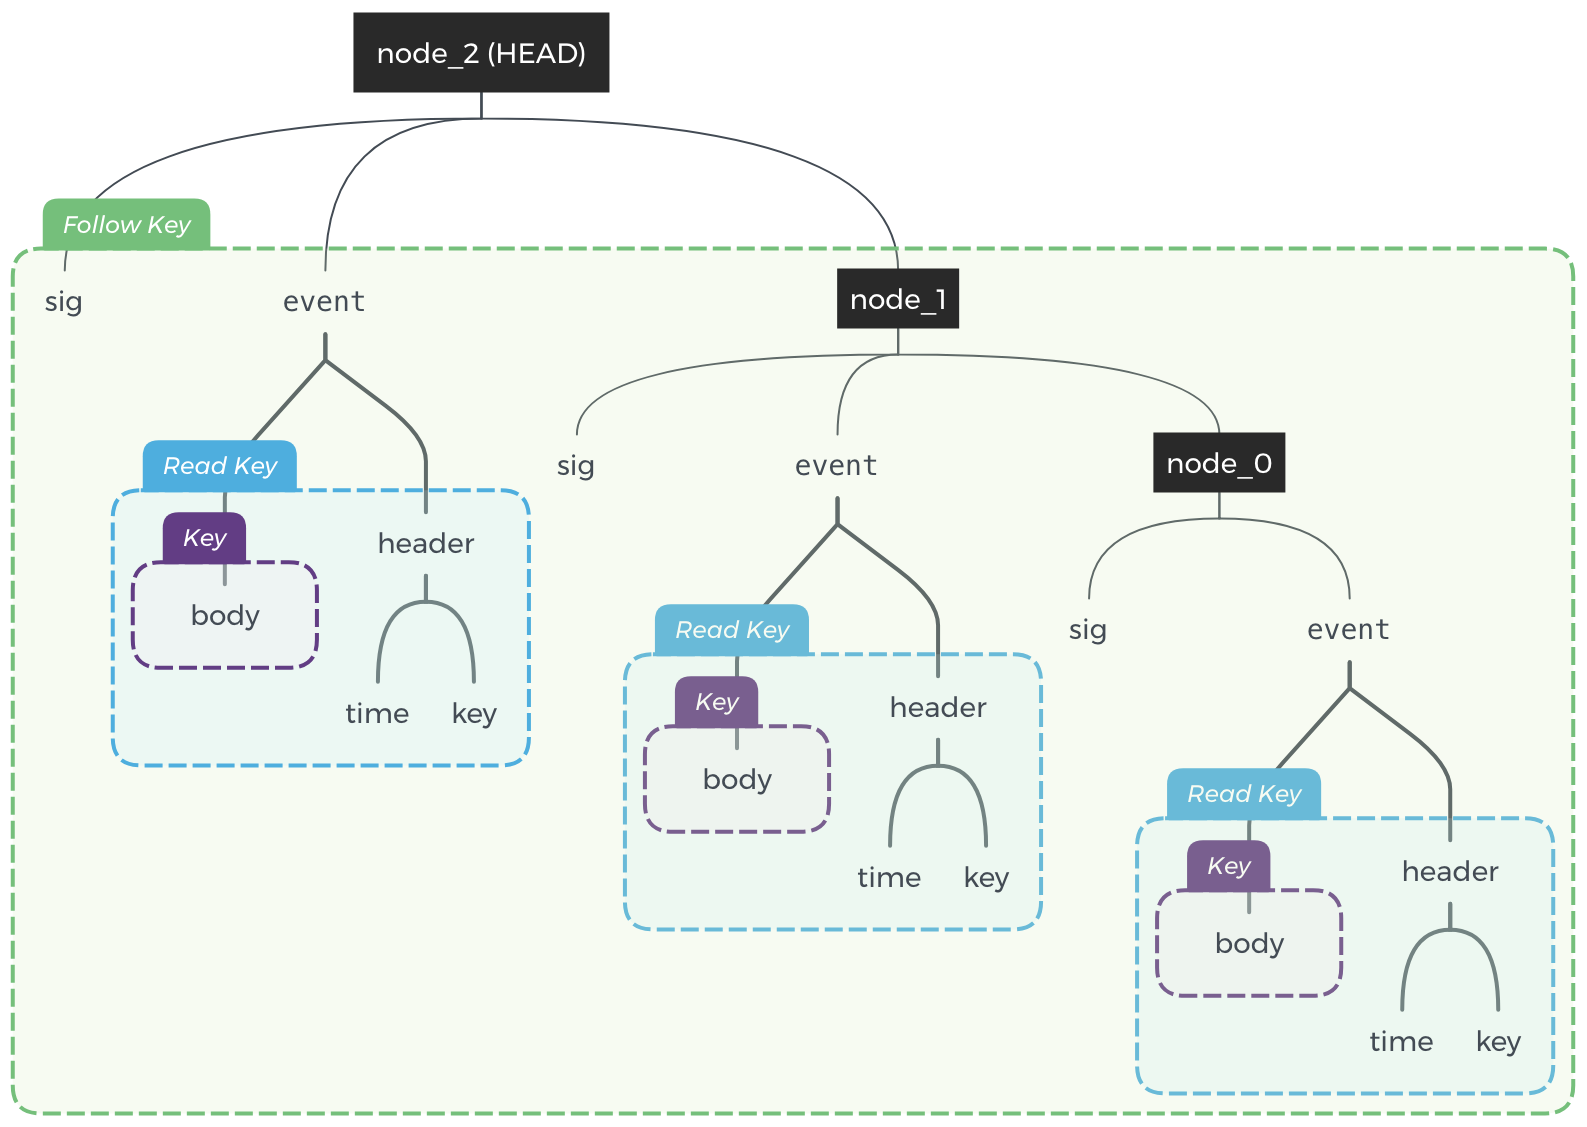
\includegraphics[width=\linewidth]{figures/Event_Log_With_Encryption.png}
  \caption{The three layers of Log Event encryption.}
  \label{fig:LogEncryption}
  \end{minipage}
\end{figure*}

\begin{example}
\begin{lstlisting}
// KeyBook stores log keys
type KeyBook interface {
   PubKey(thread.ID, peer.ID) ic.PubKey
   AddPubKey(thread.ID, peer.ID, ic.PubKey) error
   PrivKey(thread.ID, peer.ID) ic.PrivKey
   AddPrivKey(thread.ID, peer.ID, ic.PrivKey) error
   ReadKey(thread.ID, peer.ID) []byte
   AddReadKey(thread.ID, peer.ID, []byte) error
   FollowKey(thread.ID, peer.ID) []byte
   AddFollowKey(thread.ID, peer.ID, []byte) error
}
\end{lstlisting}
\caption{A KeyBook storing log keys.}
\end{example} \label{ex:KeyBook}


Textile Logs are designed to be shared, composed, and layered into datasets. Therefore, Logs are encrypted by default in a manner that enables access control (see Section  \ref{sec:AccessControl}) and the Follower mechanism discussed in the previous section.

\begin{definition}
(Identity Key). Every Log requires an asymmetric key-pair that determines ownership and identity. The private key is used to sign each Event added to the Log, so down-stream processes can verify the Log’s authenticity. Like IPFS peers, the public key of the Log is used as an identifier (Log ID).
\end{definition}

The body, or content of an event, is encrypted by a Content Key. Content keys are generated per-content and never reused. The Content key is distributed directly in the header of the Event Block. We define the Content Key as follows,

\begin{definition}
(Content Key). The Content key is a variable-format key used to encrypt the body (content) of an event. This key can be symmetric, asymmetric, or possibly non-existent in cases where encryption is not needed. One of two common encryption choices will typically be used per event, 
\begin{enumerate}
\item \label{Perf1}When broadcasting events to many possible recipients, a single-use symmetric key is generated per unique content body.
\item \label{Perf2}When sending events to specific recipients, the recipient's public key can be used to restrict access from all others.
\end{enumerate}
\end{definition}

If a single-use symmetric key is used for the Content key, it is necessary to distribute each new key to users by including it in the header of the Event Block. Therefore, the Event Block itself is further encrypted using a Read key. The Read key is not distributed within the Log itself but is distributed to any peers to grant them access to the content of the Log. 

\begin{definition}
 (Read Key). The Read key is a symmetric key created by the Log owner and used to encrypt the Content Key in each event.
\end{definition}

Finally, the encrypted Event Block, its signature, and the IPLD linkage(s) from an Event to its antecedents are encrypted together using a Follow key. Follow keys allow Logs to be followed by peers on the network who do not have access to any content within the event, and can only see signatures and linkage(s) between Events.

\begin{definition}
(Follow Key). The Follow key is a symmetric key created by the Log owner and used to encrypt the entire event payload before adding the event to the Log.
\end{definition}

Much like the Log address book, Log keys are stored in a key book (see Example \ref{ex:KeyBook}).

\subsection{Threads}

In Textile, the interface to Logs is managed as a Thread. As mentioned previously, a Thread is a collection of Logs on a given topic. Threads are an event-sourced, distributed database, and can be used to maintain a single, collaboratively edited, watched, or hosted dataset across multiple Peers. Threads provide the mechanism to combine multiple Logs from individual authors into singular shared states through the use of either cross-Log sequencing (e.g. using a Bloom Clock, Merkle-Clock, or Hybrid Logical Clock [ref]) or a CRDT (see section xx).

\subsubsection{Identity}

A unique Thread IDentity (TID) is used to group together Logs which compose a single dataset and as a topic identifier within Pub/Sub-based synchronization. TIDs are defined with the following format:

\begin{figure}
  
\includegraphics[width=\linewidth]{boat.jpg}
  \caption{The thread id formula.}
  \label{fig:boat1}
\end{figure}

TIDs share some similarities with UUIDs [ref] (version and variant) and IPFS-based CIDs and are multibase encoded [ref] for maximum forward-compatibility.

\begin{definition}
(Multibase Prefix). The encoding type used by the multibase encoder. 1 byte.
\end{definition}

Base32 encoding is used by default. However, any multibase-supported string encoding may be used.

\begin{definition}
(Version). ID format version. 8 bytes max. This allows future version to be backwards-compatible.
\end{definition}

\begin{definition}
(Variant). Used to specify thread-level expectations, like access-control. 8 bytes max. See section 3.2.2 for more about variants.
\end{definition}

\begin{definition}
(Random Number). A random number of a user-specified length. 16 bytes or more.
\end{definition}

\subsubsection{Variants}

Certain ID variants may be more appropriate than the others in specific use cases. For example, Textile provides an access-controlled Thread variant, which supports various collaborative structures — e.g., social media feeds, shared documents, blogs, photo albums, etc.


\begin{definition}
(Raw). This variant declares that consumers are not expected to make additional assumptions. This is the default variant. 
\end{definition}

Example (V1, 128 bit): `bafkxd5bjgi6k4zivuoyxo4ua4mzyy`


\begin{definition}
(Access-Controlled): This variant declares that consumers should assume an access control list is composable from Log Events. The ACL represents a permissions rule set that must be applied when reading data (see Section  \ref{sec:AccessControl}).
\end{definition}

Example (V1, 256 bit): `bafyoiobghzefwlidfrwkqmzz2ka66zgmdmgeobw2mimktr5jivsavya`

\subsubsection{Log Synchronization} \label{sec:LogSync}

Log Writers, Readers, and Followers synchronize the state of their Logs by sending and receiving Events. Inspired by Git [ref], a reference to the latest Event in a Log is referred to as the Head (or sometimes the root). When a new Event is received, Readers and Followers simply advance their Head reference.

Regardless of the network protocol, Events are transported between Peers in a standardized Event Envelope:

\begin{definition}
(Event Envelope). An over-the-wire message containing an Event and the sender’s signature of the Event.
\end{definition}

A new Thread is created by generating a TID and Log. The Log’s creator is the Writer, meaning it has possession of the Log’s Identity, Read, and Follow keys. All of these keys are needed to compose Events. At this point, the Thread only exists on the Writer’s machine. Whether for collaboration, reading, or following, the process of sharing a Thread with other Peers starts by authoring a special Event called an Invite, which contains a set of keys from all of the Thread’s Logs, called a Key Set.

\begin{definition}
(Invite). An Event containing a mapping of Log IDs to Key Sets, which can be used to join a Thread. Threads backed by an access control list (see Section  \ref{sec:AccessControl}) will also include the current ACL for the Thread in an Invite. This enables Peers to invite others to only read or follow a Thread, instead of becoming a full-on collaborator, i.e., a new Log Writer.
\end{definition}

\begin{definition}
(Key Set). A set of keys for a Log. Depending on the context, a Key Set may contain the Follow and Read key, or just the Follow key. Encrypted with the recipient’s public key.
\end{definition}

The Invite is authored in the sender’s Log. Because the recipient does not yet have this Log’s Key Set, the Event is encrypted with the recipient’s public key. If the recipient accepts the Invite, they will author another special Event called a Join in a new Log of their own.

\begin{definition}
(Join). An Event containing an invitee’s new Log ID and Key Set, encrypted with the Key Set of the inviting Peer’s Log.
\end{definition}

For a Join to be successful, all Log Writers must receive a copy of the new Key Set so they can properly handle future Events in the new Log. Instead of encrypting a Join with the public key of each existing Writer, we can encrypt a single Join with the Key Set of the inviting Peer’s Log, which the other Writers also have.

Once a Peer has accepted an Invite, it will receive new Events from Log Writers. In cases where the invitee becomes a collaborator, i.e., a Writer, it is also responsible for sending its own Events out to the network.\\

\textbf{Sending} \\

Sending is performed in multiple phases because, invariably, some Thread participants will be offline or unresponsive. 

\begin{enumerate}
\item \label{Perf1}New Events are pushed directly to the Thread’s other Log Writers.
\item \label{Perf2}New Events are pushed directly to the target Log’s Follower(s), who may not maintain their own Log.
\item \label{Perf3} New Events are published over Libp2p’s gossip-based Pub/Sub infrastructure using TID as a topic, which provides potentially unknown Readers or Followers with an opportunity to consume Events in real-time.
\end{enumerate}

Step 2 above allows for additional push mechanisms, as followers with public IP addresses become relays:

\begin{enumerate}
\item \label{Perf1}New Events may be pushed to web-based participants over a WebSocket.
\item \label{Perf2}New Events may be pushed to the Thread’s other Log Writers via federated notification services like Apple Push Notification Service (APNS) [ref], Google Cloud Messaging (GCM) [ref], Firebase Cloud Messaging (FCM) [ref], and/or Windows Notification Service (WNS) [ref].
\item \label{Perf3} New Events may trigger web-hooks [ref] enabling complex workflows (see Section X below).\\
\end{enumerate}

\textbf{Receiving} \\

Similar to sending, there are multiple paths to receiving new Events that together maximize connectivity between Peers who are often offline or unreachable.

\begin{enumerate}
\item \label{Perf1}Log Writers can receive Events directly from the author.
\item \label{Perf2} Events can be pulled from replicating Followers via HTTP, libp2p, RSS, Atom, etc.
    a. In conjunction with push over WebSockets (2a above), this method provides web-based Readers and Followers with a reliable mechanism for receiving Log Events.
\item \label{Perf3} Writers and readers can receive new Events via a Pub/Sub subscription at the TID.
\end{enumerate}

<insert diagram of pulling from a replicating Follower)

\subsubsection{Log Replication}

Replication of Thread data can happen by duplicating/syncing Log data to other Peers.

The notion of the Follow key (see Section  \ref{sec:KeysEncryption}) makes duplicating all Log Events trivial. This allows any Peer in the network to be granted the responsibility of replicating data from another Peer without having read access to the data contained within the Log entries. This type of Log replication can act as a data backup mechanism. It can also be used to build services that react to Log Events, potentially pushing data to disparate, non-Textile systems, especially if the replication service is granted read access to the Log Events (see section  \ref{sec:LogSync}).

\subsection{Thread Views} \label{sec:threadviews}

The use of well-established design patterns from the CQRS+ES (and related) literature means the Threads protocol can provide the foundation for many higher-level concepts and technologies. For instance, the public application programming interface (API) for a Thread provides several features that you would expect when operating on a dataset or table within a database. Indeed, each Thread is defined by a unique ID (its Identity), and provides facilities for access control and permissions, networking, sharing, invites, and more.

Like many CQRS-based systems, the “public” API for Threads revolves around the concept of Views (see background section xxx), which are used to optimize queries on the local event store. A key feature of Views is they are completely disposable, because they can be entirely rebuilt from the source event store. In Threads, Views are updated by subscribing to specific Event(s), and applying a Reducer function that is used to update the View state (which may be materialized to local persistent storage). This simple subscription system provides a flexible framework for building complex View-driven application logic.

\subsubsection{Default Views}

The core Textile Threads interfaces are also exposed via interfaces compatible with existing datastores and/or communications systems. These simple, public-facing APIs will be comfortable to application developers looking to leverage highly-distributed systems that connect user-controlled data, with minimal configuration and maximum interoperability. In the remainder of this section, we highlight a number of planned database abstractions to provide further utility to developers interested in building on Textile’s Threads protocol.\\

\textbf{Databases} \\

A key/value store built on top of Threads can map database `Put` operations into internal `KeyValueUpdated` events. These Events would then operate on a map-like view model, via an internal “projection“ (reducer function). The key/value view could be persisted or kept in-memory, and would be directly queried via a corresponding `Get` operation. Because Textile uses ES patterns, a `Del` operation would simply lead to an internal `KeyValueDeleted` event, marking the key/value pair for removal from the key/value materialized view.

\begin{example}
\begin{minipage}{.45\textwidth}
\begin{lstlisting}
type TextileKVStore interface {
  Put(key string, value interface{}) error
  Get(key string) (interface{}, error)
  Del(key string) error
}
\end{lstlisting}
\end{minipage}
\caption{The Key-Value store interface.}
\end{example} \label{ex:KVStore}

Similar abstractions could (and will) be used to implement additional database types and functions. The key here is to create simple, higher-level interfaces on top of Textile Threads that simplifies dealing with events and data, but exposes the underlying event sourced data for customizing as needed. Developers should not have to learn a whole new set of terms and tools to take advantage of Textile’s Threads capabilities. Other database abstractions include a no-sql style document store for storing and indexing arbitrary structs and/or JSON documents:

\begin{example}
\begin{minipage}{.45\textwidth}
\begin{lstlisting}
type TextileDocumentStore interface {
  Put(doc Inedexable) error
  Get(key string) (Indexable, error)
  Del(key string) error
  Query(query Query) ([]Indexable, error)
}
\end{lstlisting}
\end{minipage}
\caption{The Document store interface.}
\end{example} \label{ex:AddrBook}

Where `Indexable` can be satisfied by any structure with a  `key` field and and `Query` is taken from the `go-datastore` interface library [ref] or similar. Tables, feeds, counters, and other simple stores can also be built on Threads, and may require ORM-based solutions to support persistence to certain backing stores. Each database style will be implemented as a standalone software library, allowing application developers to pick and choose the solution most useful to the application at hand. Similarly, more advanced applications could be implemented using a combination of database types, or by examining the source code of these “example“ libraries.\\

\textbf{CRDTs} \\

Eventually consistent, CRDT-based stores can also be implemented on top of Threads. CRDT-based stores are particularly useful for managing Views of a document in a multi-peer collaborative editing environment (like GoogleDocs [ref] or similar). For example to support offline-first, potentially concurrent edits on a shared JSON document, one could implement a JSON CRDT datatype [ref] that applies updates on a JSON document View model. Libraries such as Automerge [ref] provide useful examples of reducer function that make working with JSON CRDTs relatively straightforward, and implementations in other programming languages are also available. A practical example of using a JSON CRDT in Textile is given in section 3.4, where it is used to represent updates to an ACL document for an access-controlled Thread implementation.\\

\textbf{Application State} \\

For application developers familiar with common state management issues, tools such as Redux provide an opinionated framework for making state mutations predictable by imposing certain restrictions on how and when updates can happen. In fact, Redux builds on concepts from CRQS and ES itself [ref], and combines them with three core principals [ref]: 1) that the entire “state“ of an application should be stored in a single “store“, 2) where the only way to change the state is to emit an “action“ (or event), which 3) transforms the application state using a “pure“ (i.e., zero side effects) reducer function (projection). In practice, Redux doesn't care how a developer persists the application state, which means a Thread’s event store and read-only materialized views are excellent candidates. This focus on unidirectional data flow in perfectly in line with architecture proposed in this paper, and as such, a compatible Redux API will be built on top of Textile Threads.


\subsection{Thread Extensions}

At an abstract level, the Textile protocol provides a highly distributed framework for building shared, offline first, datastores that are fault tolerant, eventually consistent, and scalable. Any internal implementation details of a compliant Threads “client“ may use any number of well-established design patterns from the CQRS+ES (and related) literature to “extend“ the Threads protocol with additional features and controls. Some examples of extensions that are included by default in Textile’s Threads implementation are outlined in this section to provide some indication of the extensibility of Threads.

\subsubsection{Snapshots and Compaction}

Snapshots are simply the current state of a View at a given point in time. They can be used to rebuild the state of a view without having to query and re-play all previous events. When a Snapshot is available, a Thread Peer can rebuild the state of a given View by replaying any events generated since the latest Snapshot (with a corresponding reduction in the total number of events that need to be processed) using the View’s Reducer function. Multiple peers processing the same Log could create a Snapshot every 1000 events and be guaranteed to create the exact same Snapshot because each Peer’s Event counts are identical. 

In practice, Snapshots are written to their own Event log and stored locally. They can potentially be synced (see section 3.2.4) to other peers as a form of data backup or to optimize state initialization when a new peer starts participating in a shared Thread (saving disk space, bandwidth, and time). They can similarly be used for initializing state during recovery.

Compaction can similarly speed up re-hydration of state, and is useful when only the latest Event per Event type is required. In addition to being used as a starting point for initialization and recovery, compacted logs can be used to replace the Log from which they were created in order to free up local disk space. In Textile, compaction becomes much easier because a log only has one writer and conflicts are not possible. In practice, Log compaction is a local-only operation (i.e., other Peers do not need to be aware that Compaction was performed).

\subsubsection{Access Control} \label{sec:AccessControl}

One of the most important properties of a shared data model is the ability to apply access control rules. There are two forms of access control possible in Threads, Sequence-level ACLs and Thread-level ACLs. Thread-level access control lists (ACLs) allow creators to specify who can follow, read, write, and delete Thread data. Similarly, sequence-level ACLs provide more granular control to Thread-writers on a per-sequence (see Definition XXX) basis. Both types of ACLs are materialized views, or more specifically, JSON CRDT documents, built from Log Events (see section 3.3.2 for details). ACLs implemented as JSON documents provides two advantages over static or external ACL rules (although static and external ACLs are also possible). First, ACLs are fully mutable, allowing developers to create advanced rules for collaboration with any combination of readers, writers, and followers. Second, because ACLs are JSON documents, ACLs can specify their own editing rules (i.e. allowing multiple Thread participants to modify the ACL) in a self-referencing way.

\begin{definition}
(Sequence). An Event Sequence is a series of ordered events referring to a specific entity or object. For example, an ACL JSON document is a single entity made up of a sequence of Thread Events. A Sequence might have a unique UUID (.e.g, id =bafykrq5i25vd64ghamtgus6lue74k) as in the example below.
\end{definition}

fixidexampleabove

Textile’s Threads includes ACL management tooling based on a Role-based access control [ref] pattern, wherein individuals or groups are assigned roles which carry specific permissions. Roles can be added and removed as needed. Textile ACLs can make use of five distinct roles: No-access, Follow, Read, Write, and Delete.

\begin{definition}
(No-access). No access is permitted. This is the default role.
\end{definition}

\begin{definition}
(Follow). Access to Log Follow Keys is permitted. Members of this role are able to verify Events and follow linkages. The Follow role is used to designate a “follower” peer for offline replication and/or backup.
\end{definition}

\begin{definition}
(Read). Access to Log Read Keys is permitted in addition to Follow Keys. Members of this role are able to read Log Event payloads.
\end{definition}

\begin{definition}
(Write). Members of this role are able to author new Events, which also implies access to Log Follow and Read Keys. At the Thread-level, this means authoring a Log. At the document-level, the Write role means that Events in this Log are able to target a particular document.
\end{definition}

\begin{definition}
(Delete). Members of this role are able to delete Events, which implies access to Log Follow Keys. In practice, this means marking an older Event as “deleted”.
\end{definition}

Below is a typical Thread-level ACL JSON document (where id is a unique id), which could be persisted to a local document store as part of a materialized view.

todo: fixidexampleabove 

todo: change code type below

\begin{example}
\begin{minipage}{.45\textwidth}
\begin{lstlisting}[language=json,firstnumber=1]
{
  "_id": "bafykrq5i25vd64ghamtgus6lue74k", // TID
  "default": "no-access",
  "peers": {
    "12D..dwaA6Qe": ["write", "delete"],
    "12D..dJT6nXY": ["follow"],
    "12D..P2c6ifo": ["read"],
  }
}
\end{lstlisting}
\caption{blahblah}
\end{minipage}
\end{example}

The `default` key states the default role for all network peers. The `peers` map is where roles are delegated to specific peers. Here, `12D..dwaA6Qe` is likely the owner, `12D..dJT6nXY` is a designated follower, and `12D..P2c6ifo` has been given read access.

 A Thread-level ACL has it’s own document ACL, which also applies to all other document ACLs:

\begin{example}
\begin{lstlisting}[language=json,firstnumber=1]
{
  "_id": "bafykrq5i25vd64ghamtgus6lue74k-acl", // TID-acl
  "default": "no-access",
  "peers": {
    "12D..dwaA6Qe": ["write", "delete"],
  }
}
\end{lstlisting}
\caption{Blahblah}
\end{example}

This means that only `12D..dwaA6Qe` is able to alter the access-control list.

\section{Conclusion}

In this paper, we described the challenges and considerations when attempting to create a protocol suitable for large-scale data storage, synchronization, and use in a distributed system. We identified six requirements for enabling user-siloed data: flexible data formats, efficient synchronization, conflict resolution, access-control, scalable storage, and network communication. We presented a novel solution to satisfy each of these six requirements. We have introduced a solution that extends on IPFS and prior research done by Textile and others, which we term Threads. Threads are a novel data architecture that builds upon a collection of protocols to deliver a scalable and robust storage system for end-user data. 

We show that the flexible core structure of single-writer append-only logs can be used to compose higher-order structures such as Threads, Views, and/or CRDTs. In particular, we show that through the design of specific default Views, we can support important features such as access control lists. The Threads protocol described here is flexible enough to derive numerous specific database types (e.g. key/value stores, document stores, relational stores, etc) and model an unlimited number of applications states. The cryptography used throughout Threads will help shift the data ownership model from apps to users. 

TABLE

\subsection{Future Work}

The research and development of Textile Threads has highlighted several additional areas of work that would lead to increased benefits for users and developers. In particular, we have highlighted network services and security enhancements as core future work. In the following two sections, we briefly outline planned future work in these critical areas.

\subsubsection{Enhanced Log Security}

Threads change the relationship between a user, their data, and the services they connect with that data. The nested, or multi-layered, encryption combined with powerful ACL capabilities create new opportunities to build distributed services, or Bots, on a network of Textile peers. Based on the Follow key now available in Threads, Bots would be able to relay, replicate, or store data that is synchronized via real-time updates in a trust-less way [ref]. Bots can additionally enhance the IPFS network by providing a framework to build and deploy many kinds of trust-less or trusted services. Examples include simple archival, caching and republishing Bots. Other examples include payment, re-encryption, or bridges to Web 2.0 services to offer decentralized access to Web 2.0.

\subsubsection{Textile: The Thread \& Bot Network}

The use of a single Read and Follow key for an entire Log means that, should either of these keys be leaked via malicious (or other/accidental) means, there is no way to prevent a Peer with the leaked keys from listening to Events or traversing the Log history. Potential solutions currently being explored by Textile developers include key rotation at specific Event offsets [ref], and/or incorporating the Double Ratchet Algorithm [ref] for forward secrecy [ref].

\section{Latex Examples}

\begin{figure}
  
\includegraphics[width=\linewidth]{boat.jpg}
  \caption{A boat.}
  \label{fig:boat1}
\end{figure}

\begin{quotation}
A quote
\end{quotation}

\begin{figure*}
  
\includegraphics[width=\textwidth,height=4cm]{boat.jpg}
  \caption{This is a full width boat.}
  \label{fig:boat1}
\end{figure*}


Here is a citation models~\cite{gelenbe06}. The approach constructs

here is a ref provides performance measures of interest to the SB and to the
seller, is discussed in Section \ref{Performance} where we first
discuss how the SB can behave in order to optimise outcomes that
are in its best interest, and provide  numerical examples to
illustrate the approach and the model predictions. We then explore
how the SB can try to achieve balance and compete with the other
bidders in Section \ref{KeepUp}. Finally Section
\ref{Price-Dependent} generalises the analysis to the case where
the bidding rates depend on the current price attained in the
auction. Conclusions are drawn in Section \ref{Conclusions} where
we also suggest further work.

\begin{example*}

\begin{lstlisting}
// Node is the most basic component of a log.
// Note: In practice, this is encrypted with the Follow key.
type Node interface {
    ipld.Node

    // Event is the Log update.
    Event() Event

    // Refs are node linkages.
    Refs() []cid.Cid

    // Sig is a cryptographic signature of Event and Refs
    // created with the Log's private key.
    Sig() []byte
}

// Event represents the content of an update.
// Note: In practice, this is encrypted with the Read key.
type Event interface {
    ipld.Node

    // Header provides a means to store a timestamp
    // and a key needed for decryption.
    Header() EventHeader

    // Body contains the content of an update.
    // In practice, this is encrypted with the Header key
    // or the recipient's public key.
    Body() ipld.Node

    // Decrypt is a helper function that decrypts Body
    // with a key in Header.
    Decrypt() (ipld.Node, error)
}

// EventHeader contains Event metadata.
type EventHeader interface {
    ipld.Node

    // Time is the wall-clock time at which the Event
    // was created.
    Time() int

    // Key is an optional single-use symmetric key
    // used to encrypt Body.
    Key() []byte
}
\end{lstlisting}
  \caption{This is a full width code block.}

\end{example*}


\section{Conclusions} \label{Conclusions}
In this paper we have considered auctions in which bidders make
offers that are sequentially increasing in value by a unit price
in order to minimally surpass the previous highest bid, and
modelled them as discrete state-space random processes in
continuous time. Analytical solutions are obtained and measures
that are of interest to the SB are derived.

The measures that can be computed in this way include the SB's
probability of winning the auction, its expected savings with
respect to the maximum sum it is willing to pay, and the average
time that the SB spends before it can make a purchase. An
extension of the model that incorporates price-dependent
behaviours of the agents has also been presented.

The model allows us to quantitatively characterise intuitive and
useful trade-offs between improving the SB's chances of buying a
good quickly, and the price that it has to pay, in the presence of
different levels of competition from the other bidders.


There are interesting extensions and applications of these models
that can be considered, such as the behaviour of bidders and
sellers that may have time constraints for making a purchase, and
the possibility of the SB's moving among different auctions so as
to optimise measures which represent its self-interest. Another
interesting area of study may be to examine bidders who are
``rich'' and are willing to drive away rivals at any cost, and who
may create different auction environments for bidders that have
significantly different levels of wealth. Yet another area of
interest concerns auctions where items are sold in batches of
varying sizes, with prices which depend on the number of items
that are being bought.

\ack{This research was undertaken as part of the ALADDIN
(Autonomous Learning Agents for Decentralised Data and Information
Networks) project and is jointly funded by a BAE Systems and EPSRC
(Engineering and Physical Research Council) strategic partnership
(EP/C548051/1).}


\nocite{*}

\bibliographystyle{compj}
% \bibliography{ModellingBidders}
\input{whitepaper.bbl}


\end{document}
